\section{Introduction}

\subsection{Problem Statement \redtext{(what is the problem to be solved?)}}
We develop a centralized method for estimating missing data in sensor network datasets, a procedure which is crucial for subsequent analysis.
Missing data imputation (a term from Statistics) has a long history, and while there are many existing algorithms which estimate missing sensor data (as documented in Section \ref{sec:rw}), few of these take advantage of the time and inter-sensor correlations inherent in the WSN datasets.
Furthermore, distributed approaches~\cite{xiao2006space,nowak2003distributed} are often limited to providing estimations or decisions based on sensors in the immediate neighborhood and rely on the deployed sensors having adequate computational power to perform such calculations.
Not suffering from these issues, the centralized approach we have taken enables a global solution (utilizing all observations available from the sensor network) and provides a vital backdrop for our novel highly-accurate sensor network data imputation technique.

%\subsection{Relevance (why is WSN dataset analysis an important topic?)}
%The increasing pervasiveness of Wireless Sensor Network (WSN) deployments is reflected by the recent coinage of terms such as ``Internet of Things'' and ``Machine-to-Machine'' to describe this growing revolution~\cite{ashton2009internet,gershenfeld2004internet,nokia2004machine,lawton2004machine}.
%Facilitated by a sharp reduction in hardware costs~\cite{estrin2000special}, this growing trend (beyond providing for the admission of new phrases into the vernacular) has led to an explosion in the amount and variety of sensor network data in need of study.
%For this reason, analysis of WSN data has garnered much attention in recent years~\cite{balazinska2007data}.

\subsection{Motivation \redtext{(why is data imputation needed for WSN datasets?)}}
Wireless Sensor Networks are especially susceptible to interference, power failure, and other environmental and communications ailments which lead to data loss.
One important area of WSN data analysis, however, is the application of machine learning algorithms to discriminate between or predict the occurrence of events within the sensor network deployment environment.
Many of these approaches (e.g.\ Support Vector Machine (SVM)~\cite{vapnik2000nature}, Multiple Regression (MR), etc.) require complete datasets are unable to deal with missing values.
The filling of these missing data values (in Statistics, known as Data Imputation) is thus a vital tool in the preparation of WSN data for subsequent analysis. 
Because subsequent analyses depend on accurate sensor data to draw quality conclusions or predictions, improvement in missing sensor data estimation methodology can directly lead to better solutions to sensor network deployment objectives.

\subsection{Background \redtext{(what solutions currently exist?)}}
Data imputation techniques as applied to WSN datasets can be divided into three categories:
temporal methods (i.e.\ estimation using the observations from the target sensor at nearby time-steps), 
spatial methods (i.e.\ estimation using neighboring sensor node observations), 
%heterogeneous sensor methods (i.e.\ like spatial, however now considering sensors of different types),
and hybrid methods.

%\subsubsection{Temporal Methods}
The feasibility of estimating missing sensor observations based on historical data is grounded by the known temporal correlation in WSN data~\cite{akyildiz2004exploiting}.
Moreover, where there is a potential for global communication issues to affect the availability for sensor node observations \emph{en masse} during a given duration of time, utilizing spatial correlations as a basis for estimation may be not be possible.
Temporal imputation methods include observed data mean~\cite{madden2005tinydb,setz2009combining}, last seen, and linear interpolation.
These methods suffer, however, when there are long temporal gaps of data for a given sensor (i.e.\ as can happen when intermittent communications starvation occurs in large WSNs).
As a result, the usefulness of temporal imputation methods drop rapidly as the number of consecutively missing packets becomes large.

%\subsubsection{Spatial Methods}
Where spatial information is available for deployed sensor nodes, this information may be used to enforce a correlation among of neighboring sensor observations.
Methods which exploit this approach include associations rule mining~\cite{le2005estimating,jiang2007estimating} and weighting functions of nearby sensors~\cite{li2008spatial,li2008data,pan2010k}.
Generally, methods which rely solely on the spatial imputation approach suffer from the inability to estimate missing data when global sensor outages occurs such that neighboring sensor values also become unavailable.

\begin{figure}[H]
\centering
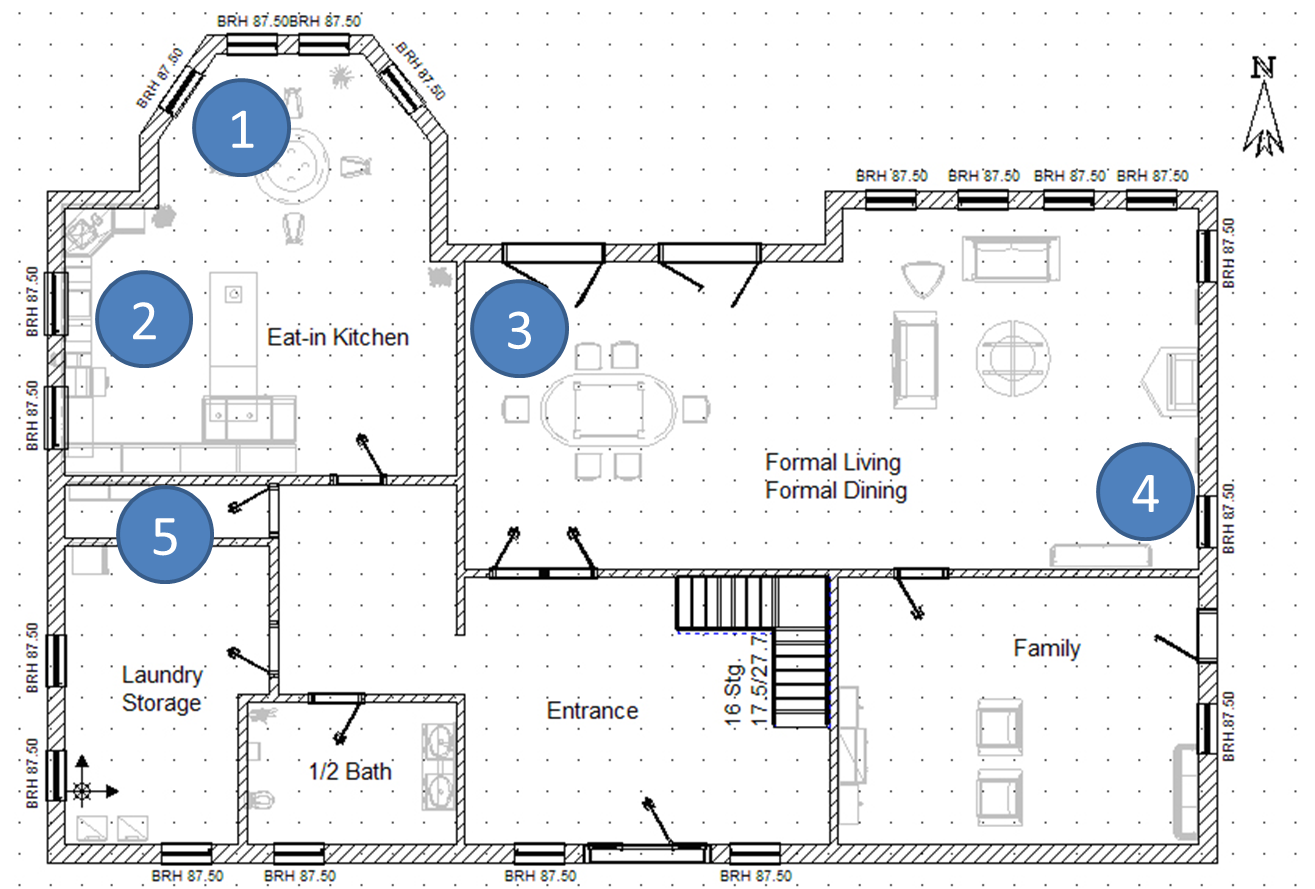
\includegraphics[scale=0.35]{house_floorplan.png}
\caption{Example home floorplan showing five deployed temperature sensors} \label{house_floorplan}
\end{figure}

Spatial methods also fail to take into account barriers or other sources of sharp environmental gradients which may deter the usage of spatial information as a first-order inter-sensor node correlation approximation.
For example, in Figure \ref{house_floorplan}, we find sensors $1$ \& $2$ deployed in the kitchen, nearby the stove and outside window, respectively. While these sensors are close in proximity, assuming the stove is in use and the temperature outside is cold, there may be a large temperature difference between these two sensors despite their close proximity.
Similarly, sensors $2$ \& $5$ may be quite uncorrelated despite their relative proximity due the wall between them and the presence of kitchen or laundry appliance use.
On the other hand, sensors $3$ \& $4$, while located further from one another may be quite correlated despite their remote placement as they are both near an outside wall and both within the same room.
%For instance, a sensor deployed in close proximity to a furnace and one deployed nearby, but beneath an air-conditioning vent, may be only weakly correlated by spatial information.
%There is also the corollary possibility of a pair of temperature sensors deployed quite distance from one another, yet having a strong correlation due to well-circulated air flow between the two.
The calculation of inter-node signal strength or line of sight distance between nodes can help to mitigate the issues of spatially-based imputation, though not a complete remedy.
In the end, the incorporation of spatial information can lead to worse imputation results as non-existent (or at least inconsistent) correlations are imposed between sensors.

Certain methods consider not strictly the distance between sensors, but instead establishes a ``neighborhood of influence'' whose size becomes a tuning parameter of this approach, which adds to the complexity of this approach.

%\subsubsection{Heterogeneous Sensor Methods}
%\redtext{more here!}

%\subsubsection{Hybrid Methods}
Hybrid models are also a studied approach.
This topic is covered later in the paper. %for now, it was moved to discussion!

%Hybrid methods of temporal and spatial approaches are less common in the literature.
%For example, the average of the temporal approach of linear interpolation and the spatial approach of multivariate regression has been reported[8].
%Strictly speaking, this approach can be thought of as an ensemble approach between the two methods rather than a fully-integrated approach which considers both temporal and spatial aspects of WSN data.

%\subsection{Research Gap Identification (why are current approaches inadequate?)}
%Accurate imputation of missing sensor network observations is crucial to allow for effective subsequent analysis.
%While there are many existing algorithms which estimate missing data (as documented in the following Related Works section), few of these take advantage of the time and space dependencies inherent in the WSN datasets during the data imputation process.
%As a result, the accuracy of such approaches is limited.

\subsection{Method Overview \redtext{(what is our approach to bridge the research gap?)}}

\begin{figure}[H]
\centering
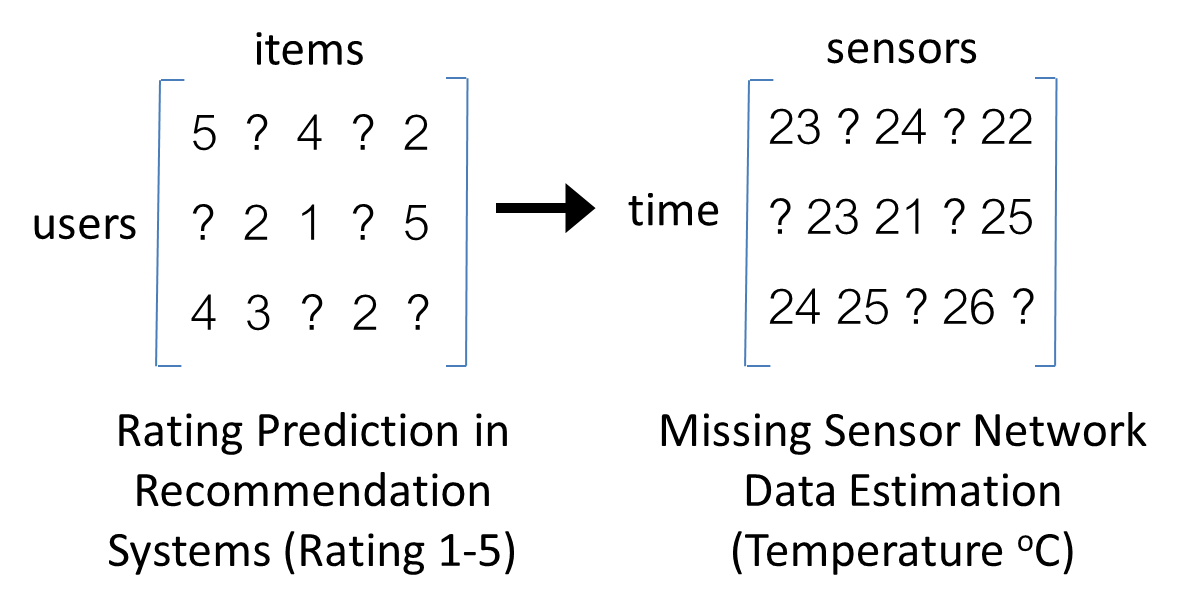
\includegraphics[scale=0.35]{recommend_imputation.png}
\caption{Bridge from Recommendation Systems to Missing Sensor Network Data Estimation} \label{recommend_imputation}
\end{figure}

In our work, we employ a novel collaborative-filtering (CF) approach to WSN data imputation inspired by the field of Recommendation Systems.
In typical CF approaches, the elements of interest are users and items, whereas WSNs are sensor node and time-steps.
Applying standard CF techniques, a sensor reading at a given time-step may be estimated much like a user rating for a given item.
Clearly a sensor reading at a given time will be correlated with itself and its neighbors at times close to that given.
It is this insight and the potential integration with CF methods which has driven the current work.
In particular, we focus on Matrix and Tensor Factorization, providing a novel method to augment these well-established techniques to exploit the temporal relationship in the sensor data.
%Our method, in addition, is able to utilize the spatial information of the sensor nodes where the correlations cannot be learned from the sensor data itself.
We are also able to exploit heterogeneous sensor information in our solution, which few other methods have proposed a proper way to incorporate.
Our method incorporates these heterogeneous sensor signals (for example, estimating the temperature at a given sensor node utilizing the humidity, temperature, and light trends from other sensors in the network) to provide a better estimation of the missing data than approaches which do not benefit from this deeply comprehensive approach.

\subsection{Results Overview \redtext{(how does our method compare to the state of the art?)}}
We explore two different environmental datasets, one indoor and one outdoor.
Both datasets record temperature, humidity, and light within its deployed environment.
Each dataset has an initial missing rate (which strengthens the claim that missing data in WSNs is a common issue), to which we additionally cover known observations to use for validation and testing purposes.
Given these experimental conditions, we show that our temporal and spatial-oriented collaborative filtering approach to data imputation for WSNs performs more accurately than existing methods such as linear regression and hybrid-kNN.

\redtext{Results Overview of MF}

\redtext{Results Overview of TF}

\subsection{Contributions \redtext{(what are the novel aspects of our work?)}}
Our contributions to the body of research related to missing sensor network data estimation include:
\begin{itemize}
\item Application of the modern collaborative filtering methods of recommendation systems to the sensor network domain, specifically matrix and tensor factorization
\item Augment collaborative filtering with temporal coherence and multi-sensor signals. The reason we believe our method outperforms the results of other methods are as follows.
\begin{itemize}
\item the collaborative filtering approach utilizes latent information between sensors, e.g.\ inter-sensor correlation
\item utilizing heterogeneous sensor information (e.g.\ utilizing humidity information when estimating temperature) provides additional features which enables a more refined estimation model
\item we provide an efficient optimization method to learn the inherent model parameters effectively
\item our method provides a global solution, where all sensor observations available in the dataset can potentially aid in the estimation of a given missing observation
% (our method builds a global model incorporating intra-sensor and inter-sensor information together and directly optimizes the objective function as opposed to the piecewise combination of disparate approaches as is common in the literature.
\end{itemize}
\item Empirical study which finds that our method works well without the incorporation spatial information and that our approach can facilitate the generation of better prediction models
\end{itemize}

\subsection{Paper Organization \redtext{(how is the paper organized?)}}
The remainder of our paper is organized as follows.
Related Work is reviewed in Section \ref{sec:rw}.
In Sections \ref{sec:mf} and \ref{sec:tf} we describe our Matrix and Tensor Factorization approaches to WSN data imputation, respectively.
Sections \ref{sec:disc} and \ref{sec:conc} provide discussion of our findings and the conclusion.
